\documentclass{article}

\usepackage{graphicx}

\title{\textbf{Project Report: MUSIC PLAYER}}
\author{Ashmeet Sidhu (BT22BTECH11004)}
\date{}

\begin{document}
\maketitle


\section{\emph{Introduction}}
This report details the development of a music player application using Python. The music player allows users to play a collection of songs in a randomly shuffled order, providing essential functionalities such as pause, play, skip, and previous.

\section{\emph{Design \& Implementation}}
The music player application is built using Python, leveraging the following design and implementation details for each functionality:

\begin{itemize}
    \item \textbf{\underline{User Interface:}} The user interface is developed using the Tkinter library, a powerful Python GUI framework. Tkinter provides a rich set of tools for creating interactive graphical interfaces. It enables the placement of buttons, labels, and other widgets to enhance the user experience.
    \item \textbf{\underline{Music Library:}} The music library is established by storing song files in a designated directory. The application employs the \textbf{os} module to access the files within the library directory. It uses \textbf{os.path.join()} to construct the file paths, ensuring compatibility across different operating systems. This approach allows the music player to locate and load the songs seamlessly.
    \item \textbf{\underline{Random Shuffle:}} The random shuffle functionality is implemented using the \textbf{random} module in Python. Upon initializing the music player, it generates a random permutation of the song collection, creating a shuffled playlist. The player then loads the songs from the library using \textbf{pygame.mixer.music.load()} and plays them sequentially from the shuffled playlist.
    \item \textbf{\underline{Pause and Play:}} The pause and play functionalities are facilitated by the \textbf{pygame} library, a comprehensive multimedia framework for Python. When the user clicks the "Play" button, the music player uses \\ \textbf{pygame.mixer.music.play()} to start playing the current song. The "Pause" button triggers \textbf{pygame.mixer.music.pause()}, which temporarily halts the playback until the user resumes.

    \item \textbf{\underline{Skip and Previous:}} The skip functionality enables the user to move to the next song in the shuffled playlist. When the user clicks the "Skip" button, the music player invokes \textbf{pygame.mixer.music.stop()} to stop the current song and proceeds to load and play the next song from the shuffled playlist. The previous functionality keeps track of previously played songs, allowing the user to move back to the previous song if desired.

    
\end{itemize}

\section{\emph{Conclusion}}
In conclusion, a simple music player has been successfully developed using Python. The player allows users to play a collection of songs in a randomly shuffled order, providing essential functionalities such as pause, play, skip, and previous. The application utilizes the \textbf{Tkinter} library for the user interface, the \textbf{os} module for accessing the music library directory, and the \textbf{pygame} library for audio playback.
Overall, this project demonstrates the capability of Python in creating a simple yet functional music player application. 

\section{\emph{User Interface}}

\begin{figure}[ht]
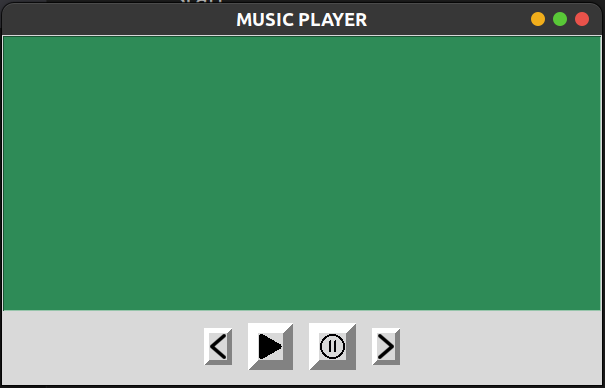
\includegraphics[width=\columnwidth]{images/figure.png}


\end{figure}



\end{document}
